\chapter{Visão Geral da Arquitectura}

A solução proposta permite gerir consentimentos digitais de forma segura, transparente e verificável, recorrendo a assinaturas digitais e certificados para garantir autenticidade e integridade.

O sistema define um fluxo de consentimento no qual cada decisão do utilizador é registada, assinada e validada, assegurando que nenhuma das partes pode manipular ou negar a informação posteriormente. Para tal, são utilizadas duas entidades principais:

\begin{itemize}
    \item \textbf{\acrlong{ds} (\acrshort{ds})}: o utilizador final que interage com a interface web do serviço e fornece o consentimento através de eventos no navegador. O DS é responsável por assinar digitalmente o consentimento antes de o enviar para validação, criando uma prova verificável da sua decisão.
    \item \textbf{\acrlong{sp} (\acrshort{sp})}: o prestador de serviços que disponibiliza o website com o \acrshort{cmp} e mantém o servidor de confiança. O SP recebe os consentimentos assinados pelo DS, valida a assinatura do utilizador, assina novamente o consentimento e mantém um registo imutável. Este registo permite auditoria, revogação e consulta futura.
\end{itemize}

O fluxo completo do sistema pode ser descrito de forma conceptual, independente da linguagem de programação utilizada:

\begin{enumerate}
    \item O \acrshort{ds} interage com o banner de consentimento na interface web fornecida pelo \acrshort{sp}.
    \item A extensão do navegador do \acrshort{ds} captura o evento, prepara o consentimento e assina digitalmente os dados.
    \item O consentimento assinado é enviado ao servidor do \acrshort{sp}, que valida a assinatura do \acrshort{ds} e cria um \textit{JSON Web Signature (JWS)} final, incorporando a assinatura do \acrshort{sp}.
    \item O JWS resultante é devolvido ao \acrshort{ds}, que pode validar a assinatura do \acrshort{sp}, garantindo que o consentimento foi corretamente registado e não foi alterado.
    \item Ambos, \acrshort{ds} e \acrshort{sp}, mantêm cópias do JWS, criando um histórico verificável e auditável.
\end{enumerate}

Desta forma, o sistema garante quatro propriedades fundamentais: 

\begin{itemize}
    \item \textbf{Transparência}: todos os passos do processo podem ser verificados pelo utilizador ou pelo prestador de serviços.
    \item \textbf{Autenticidade e Integridade}: assinaturas digitais asseguram que os consentimentos não foram alterados e que provêm das entidades corretas.
    \item \textbf{Não repúdio}: o \acrshort{ds} não pode negar a sua decisão, e o \acrshort{sp} não pode alegar que não recebeu ou validou o consentimento.
    \item \textbf{Auditabilidade}: o histórico de consentimentos permanece acessível a ambas as entidades, permitindo conformidade com requisitos legais e regulação de proteção de dados.
\end{itemize}

\section{Componentes}

O sistema é constituído por três componentes principais: a \textbf{interface web}, a \textbf{extensão do navegador} e o \textbf{servidor}.
A interface web representa o ponto de contacto direto com o utilizador e disponibiliza o \textit{banner} de consentimento.  
A extensão do navegador actua como intermediário, recebendo os eventos provenientes da interface web e tratando do processo de assinatura digital.  
Por fim, o servidor desempenha o papel de repositório de confiança, responsável por validar as assinaturas recebidas e manter o registo imutável dos consentimentos.

\section{Interacção Entre Componentes}

\quad \textbf{Interface Web $\leftrightarrow$ Extensão}
A interface web comunica com a extensão através de eventos DOM:
\begin{itemize}
    \item Deteta ações do utilizador no \textit{banner} de consentimento
    \item Transmite dados de consentimento para processamento criptográfico
    \item Recebe confirmação de sucesso para feedback ao utilizador
\end{itemize}

\textbf{Extensão $\leftrightarrow$ Servidor}

A extensão estabelece um canal seguro com o servidor:
\begin{itemize}
    \item Obtém chaves públicas RSA do servidor
    \item Envia o consentimento assinado
    \item Recebe assinatura do servidor e faz a validação da mesma
\end{itemize}

\begin{figure}[h]
\begin{center}
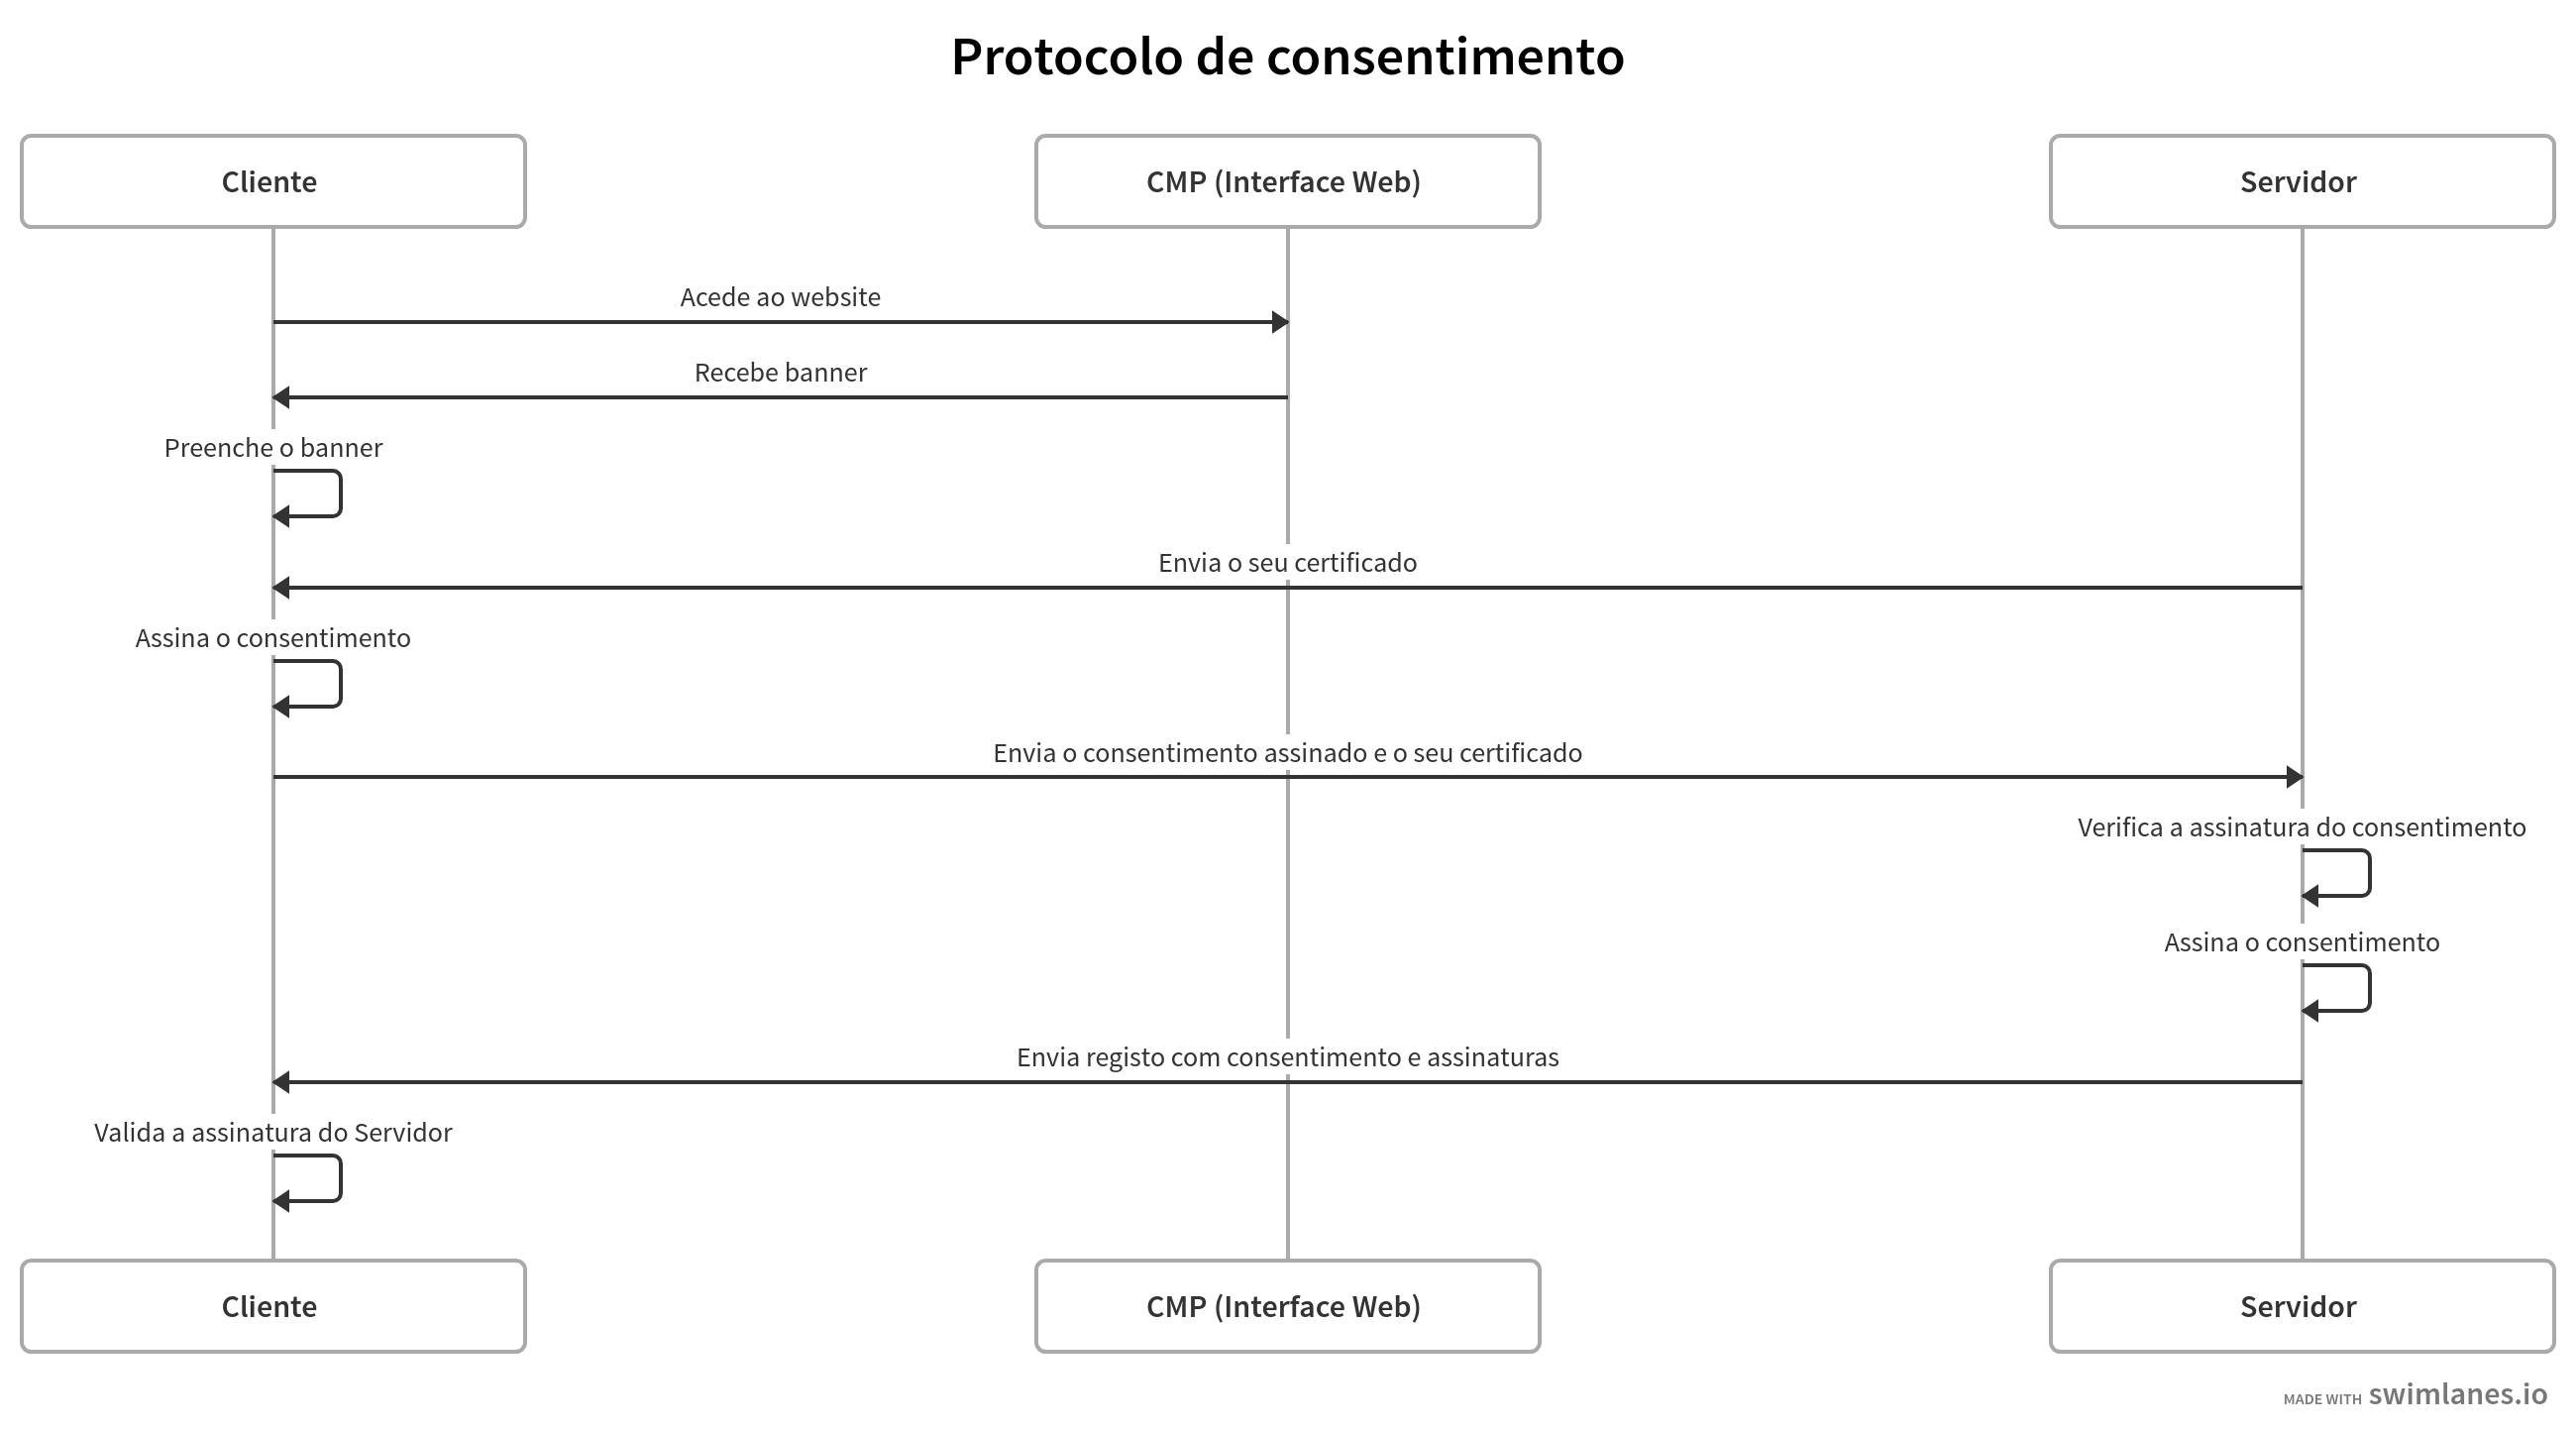
\includegraphics[width=1\textwidth]{images/swimlanes.png}
\end{center}
\caption{Diagrama do protocolo}
\label{fig:swimlane1}
\end{figure}

\newpage

\section{Lógica de Funcionamento}

A estratégia proposta assenta numa abordagem de assinaturas digitais, na qual o cliente e servidor participam ativamente na criação de um registo de consentimento verificável e imutável. Esta abordagem garante quatro propriedades fundamentais: \textbf{transparência}, na medida em que todos os passos podem ser verificados; \textbf{descentralização}, dado que nenhuma das partes detém controlo unilateral; \textbf{não-repúdio}, assegurando que os consentimentos prestados não podem ser posteriormente negados; e \textbf{auditabilidade}, uma vez que o histórico completo permanece acessível a ambas as entidades.

%Isto deveria ir para trabalho relacionado?
\section{Certificados}

Os certificados desempenham um papel fundamental na garantia de identidade e na criação de comunicações seguras. De forma simplificada, um certificado digital é um ficheiro que associa uma chave pública a uma entidade (por exemplo, um utilizador ou um servidor). Esta associação é validada por uma \acrlong{ca} (\acrshort{ca}), que funciona como uma entidade de confiança responsável por emitir e assinar certificados.

A chave privada deve permanecer confidencial, pois é utilizada para operações críticas, como a criação de assinaturas digitais. Já a chave pública, incluída no certificado, pode ser partilhada e serve para validar essas assinaturas.

A \acrshort{ca} raiz (root \acrshort{ca}) é a autoridade de topo, responsável por assinar certificados de entidades intermédias ou diretamente de clientes e servidores, como é o caso. Este mecanismo hierárquico garante que, ao receber um certificado, é possível verificar a sua autenticidade através da cadeia de confiança estabelecida pela autoridade certificadora.

\section{Assinatura Digital}

Uma assinatura digital é um mecanismo criptográfico baseado em algoritmos de chave assimétrica, concebido para garantir a autenticidade e a integridade de uma mensagem ou documento eletrónico. O seu funcionamento baseia-se em dois elementos fundamentais: a chave privada e a chave pública. A chave privada é utilizada para gerar a assinatura digital e deve permanecer secreta, acessível apenas ao titular. A chave pública é distribuída, neste caso através de certificados digitais, permitindo que qualquer entidade verifique a validade da assinatura.

Desta forma, a assinatura digital assegura três propriedades essenciais \citep{digitalsignatures}:
\begin{itemize}
    \item \textbf{Autenticidade}: confirma que a mensagem foi assinada pela entidade detentora da chave privada correspondente.
    \item \textbf{Integridade}: garante que o conteúdo não foi alterado após a assinatura.
    \item \textbf{Não repúdio}: impede que o autor negue a sua participação no processo, tornando a assinatura uma evidência legalmente relevante.
\end{itemize}

As assinaturas digitais constituem o fundamento de sistemas confiáveis de registo de consentimentos, transações financeiras e documentos eletrónicos, sendo amplamente utilizadas em padrões de segurança e infraestruturas de chave pública.

\section{Consentimento}

O consentimento do utilizador é representado como um registo estruturado que pode ser interpretado e processado de forma padronizada. Este registo deve ser interoperável, auditável e verificável, permitindo que diferentes sistemas o leiam e validem sem ambiguidade.

Para garantir estas propriedades, cada consentimento é assinado digitalmente tanto pelo utilizador como pela entidade que o recebe. A troca de certificados entre as partes possibilita a verificação mútua das assinaturas, reforçando a confiança no processo. O objecto resultante agrega informação relevante sobre as decisões do utilizador, bem como metadados necessários à validação, mantendo a integridade e autenticidade do consentimento.

Adotar um padrão estruturado para o consentimento permite:
\begin{itemize}
    \item Facilitar a integração com diferentes sistemas e aplicações;
    \item Manter um registo auditável e verificável ao longo do tempo;
\end{itemize}

\section{Benefícios da Arquitectura}

\subsubsection{Para o Utilizador}
\begin{itemize}
    \item Acesso aos seus consentimentos
    \item Capacidade de verificar a integridade dos registos
    \item Capacidade de autoria em verificação do não cumprimento
\end{itemize}

\subsubsection{Para a Organização}
\begin{itemize}
    \item Prova de consentimentos válidos
    \item Redução de riscos de conformidade
\end{itemize}
